The Semantic Web presents many opportunities for computational linguists and digital humanitarians interested in accessing, presenting, and discovering new information. However, the learning curve for the relevant technologies is steep, and first adopters may be hesitant due to lack of examples of possible uses and ignorance of useful databases for research. The Open Linguistics Working Group (OWLG) \cite{owlg4lrec}, an open community of researchers dedicated towards providing and disseminating openness in the broad field of linguistics, are creating and maintaining the Linguistics Linked Open Data (LLOD) \cite{ldl-llod, ChiarcosLOD} cloud for that purpose; to make clearly available and freely accessible multiple open databases for use by researchers and commercial companies alike. 

The LLOD is not only freely accessible to researchers, but also openly adaptable for new databases and ontologies. All databases included in the LLOD must subscribe to the Linked Open Data paradigm \citep{bernersLee2006_linkeddata}, which demands that: \begin{enumerate} \item Referred entities should be designated by using Uniform Resource Identifiers (URIs),\footnote{\url{http://tools.ietf.org/html/rfc3986}}
\item these URIs should be resolvable over HTTP,
\item data should be represented by means of specific W3C standards\footnote{\url{http://www.w3.org/}} (such as RDF),
�tem and a resource should include links to other resources.\end{enumerate} These rules facilitate information integration, and thus, interoperability, in that they require that entities can be addressed in a globally unambiguous way, that they can be accessed and interpreted, and that entities that are associated on a conceptual level are also physically associated with each other. 

Furthermore, the following criteria must be met for a new linguistic resource to be included in the LLOD cloud: \begin{enumerate}\item The data is resolvable through HTTP, \item it is provided as RDF, \item it contains links to another data set in the diagram, and \item the entire data set must be available.\end{enumerate}. At the time of writing, the LLOD has {\it draft} status, meaning that several of the resources may point only to resource metadata, although each has been promised to be uploaded and linked to the LLOD in the near future. The ontology can be viewed in Fig. \ref{f1}

\begin{figure*}[b!hpt]
\caption{The LLOD Cloud}\label{f1}
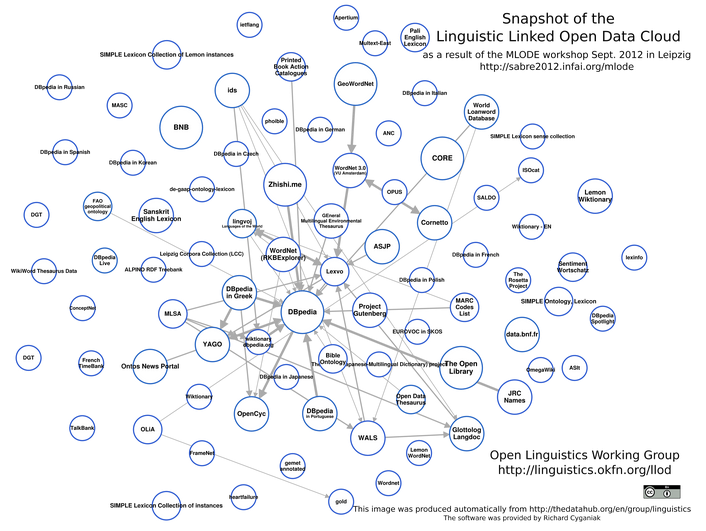
\includegraphics[width=15cm,keepaspectratio]{img/llod.png}
\end{figure*}

In order to encourage future submission of resources into the LLOD, we present a new resource - a lexical and geospatial database of languages from the Dogon family, in Western Africa. According to the iterative and incremental Linked Data Life Cycle \cite{Villazon_2011}, all linked data follows a cycle: specification, modelling, generation, publication, and exploitation (which then feeds back into future specification). Here, we go through each of these stages on the way from taking the Dogon spreadsheet to an interactive visualisation using map4rdf. We also present a visualisation using a database already in the LLOD, the World Atlas of Language Structures (WALS) \cite{Haspelmath_etal2008}, by querying for geographic information for languages using a SPARQL endpoint for the LLOD (see Littauer {\it et al.}, this issue). We hope that these efforts will encourage future researchers to both add to and utilise the LLOD for their own research.  